\documentclass[a4paper,12pt]{article} % тип документа

% Поля страниц
\usepackage[left=2.5cm,right=2.5cm,
    top=2cm,bottom=2cm,bindingoffset=0cm]{geometry}
    
%Пакет дял таблиц   
\usepackage{multirow} 
    
%Отступ после заголовка    
\usepackage{indentfirst}


% Рисунки
\usepackage{floatrow,graphicx,calc}
\usepackage{wrapfig}

%%% Работа с картинками
\usepackage{graphicx}  % Для вставки рисунков
\graphicspath{{images/}{images2/}}  % папки с картинками
\setlength\fboxsep{3pt} % Отступ рамки \fbox{} от рисунка
\setlength\fboxrule{1pt} % Толщина линий рамки \fbox{}
\usepackage{wrapfig} % Обтекание рисунков и таблиц текстом

% Создаёем новый разделитель
\DeclareFloatSeparators{mysep}{\hspace{1cm}}

% Ссылки?
\usepackage{hyperref}
\usepackage[rgb]{xcolor}
\hypersetup{				% Гиперссылки
    colorlinks=true,       	% false: ссылки в рамках
	urlcolor=blue          % на URL
}


%  Русский язык
\usepackage[T2A]{fontenc}			% кодировка
\usepackage[utf8]{inputenc}			% кодировка исходного текста
\usepackage[english,russian]{babel}	% локализация и переносы




% Математика
\usepackage{amsmath,amsfonts,amssymb,amsthm,mathtools}

%%% Дополнительная работа с математикой
\usepackage{amsmath,amsfonts,amssymb,amsthm,mathtools} % AMS
\usepackage{icomma} % "Умная" запятая: $0,2$ --- число, $0, 2$ --- перечисление


% Что-то 
\usepackage{wasysym}


\begin{document}
\begin{center}
	\footnotesize{ФЕДЕРАЛЬНОЕ ГОСУДАРСТВЕННОЕ АВТОНОМНОЕ ОБРАЗОВАТЕЛЬНОЕ 			УЧРЕЖДЕНИЕ ВЫСШЕГО ОБРАЗОВАНИЯ}\\
	\footnotesize{МОСКОВСКИЙ ФИЗИКО-ТЕХНИЧЕСКИЙ ИНСТИТУТ\\(НАЦИОНАЛЬНЫЙ 			ИССЛЕДОВАТЕЛЬСКИЙ УНИВЕРСИТЕТ)}\\
	\footnotesize{ФАКУЛЬТЕТ ОБЩЕЙ И ПРИКЛАДНОЙ ФИЗИКИ\\}
	\hfill \break
	\hfill \break
	\hfill \break
	\hfill \break
\end{center}


\begin{figure*}[h]
    \centering
    \includegraphics*[width=10cm,height=7cm,keepaspectratio]{mipt_eng_text_png.png}
    \label{fig:my_label}
\end{figure*}


\begin{center}   
    \hfill \break
	\hfill \break
	\hfill \break
	\large{Лабораторная работа № 3.1.3\\\large{\textbf{Измерение магнитного поля Земли}}}\\
	\hfill \break
	\hfill \break
	\hfill \break
	\hfill \break
	\begin{flushright}
		Баранов Даниил\\
		Группа Б02-103
	\end{flushright}
	\hfill \break
	\hfill \break
	\hfill \break
\end{center}
\hfill \break
\hfill \break
\hfill \break
\hfill \break
\begin{center}
	Долгопрудный, 2022 г.
\end{center}
\thispagestyle{empty}

\newpage

\textbf{Цель работы:} исследовать свойства постоянных неодимовых магнитов; измерить с их помощью горизонтальную и вертикальную составляющие индукции магнитного поля Земли и магнитное наклонение.

\textbf{В работе используются:} неодимовые магниты; тонкая нить для изготовления крутильного маятника; медная проволока; электронные весы; секундомер; измеритель магнитной индукции; штангенциркуль; брусок, линейка и штатив из немагнитных материалов; набор гирь и разновесов.

\section{Теоретические сведения}

Простейший магнитный диполь может быть образован витком с током или постоянным магнитом. По определению, магнитный момент $\mathfrak{m}$ тонкого витка площадью $S$ с током $I$ равен $$\mathfrak{m} = I\textbf{S},$$ где $\textbf{S} = S\textbf{n}$ - вектор площади контура, образующий с направлением тока правовинтовую систему, $\textbf{n}$ - единичный вектор нормали к площадке. Если размеры контура с током или магнитной стрелки малы по сравнению с расстоянием до диполя, то соответствующий магнитный диполь $\mathfrak{m}$ называют \textit{элементарным}, или \textit{точечным}.

Магнитное поле точечного диполя определяется по формуле, анологичной формуле для поля элементарного электрического диполя:

\begin{equation}
    \textbf{B}_\text{дип} = \frac{\mu_0}{4\pi}\left(\frac{3(\mathfrak{m} \cdot \textbf{r})\textbf{r}}{r^5} - \frac{\textbf{m}}{r^3}\right)
    \label{2}
\end{equation}


Во внешнем магнитном поле с индукцией $\textbf{B}$ на точеный магнитный диполь $\mathfrak{m}$ действует механический момент сил $$\textbf{M}=[\mathfrak{m}, \textbf{B}].$$
При этом потенциальная энергия которой обладает диполь с постоянным $\mathfrak{m}$, равна 
$$W = -(\mathfrak{m} \cdot \textbf{B}).$$
Когда диполь ориентирован вдоль внешнего поля, он находится в состоянии \textit{равновесия}. При этом \textit{устойчивым будeт} только состояние, в котором диполь \textit{сонаправлен} с полем, поскольку его потенциальная энергия достигает \textit{минимума}. При противоположной ориентации энергия будет иметь максимум, и состояние равновесия будет неустойчивым.

В \textit{неоднородном} внешнем поле выражение для энергии постоянного диполя сохраняется. При этом кроме момента сил на диполь действует ещё и сила 

\[\textbf{F} = -\nabla W = (\mathfrak{m} \cdot \nabla)\textbf{B},\]

Где $\nabla = \left(\frac{\partial}{\partial x},\frac{\partial}{\partial y}, \frac{\partial}{\partial z}\right)$ -- векторный оператор <<набла>> (оператор Гамильтона). В частности, проекция на ось $x$ имеет вид

\begin{equation*}
    F_x = \mathfrak{m}_x\frac{\partial B_x}{\partial x} + \mathfrak{m}_y\frac{\partial B_y}{\partial y} + \mathfrak{m}_z\frac{\partial B_z}{\partial z}.
\end{equation*}


Таким образом из вышесказанного следует, что \textit{свободный} магнитный диполь в неоднородном магнитном поле ориентируется вдоль силовых линий магнитного поля и втягивается в область более сильного поля, поскольку это ведёт к уменьшению энергии диполя.

Выражения выше, позволяют рассчитать силу взаимодействия магнитов с моментами $\mathfrak{m}_1$ и $\mathfrak{m}_2$. Kогда моменты двух небольших магнитов направлены вдоль соединяющей их прямой: $\mathfrak{m}_{1,2} \| \textbf{r}$, где $\textbf{r}$ - радиус-вектор между ними, они взаимодействуют с силой 
\begin{equation}
    \label{6}
    F_{12}= \mathfrak{m}_1 \frac{\partial{B_2}}{\partial{r}} = \mathfrak{m}_1\frac{\partial{(2\mathfrak{m}_2/r^3)}}{\partial{r}} = -\frac{6 \mathfrak{m}_1\mathfrak{m}_2}{r^4} \;(\text{ед}.\; \text{СГС}).
\end{equation}

(при использовании системы СИ нужно домножить на $\mu_0 / 4\pi$). Здесь магниты притягиваются, если их магнитные моменты сонаправлены, и отталкиваются, если направлены противоположно.


Если магнитные моменты направлены перпендикулярно соединяющей их прямой: $\mathfrak{m}_{1,2} \perp \textbf{r}$, то нетрудно показать, что сила их взаимодействия окажется в два раза меньшей и будет иметь противоположный знак: $$F_{12} = \frac{3\mathfrak{m}_1 \mathfrak{m}_2}{r^4}\;(\text{ед}.\; \text{СГС}).$$


\section{Экспериментальная установка}

В работе используются неодимовые магниты шарообразной формы. Важно, чтобы вещество из которого они изготовлены, было \textit{магнитожёстким} материалом и чтобы шары были намагничены однородно.


<<Манитожесткость>> материала означает, что магнитные моменты шаров в процессе работы не зменяются под действием внешних магнитных полей, т. е. шар ведет себя как постоянный (<<жесткий>>) диполь. В том числе, магнитные моменты не изменяются при контакте магнитов друг с другом.

Магнитное поле однородного намагниченного шара радиусом $R$ может быть вычислено точно. На расстояниях $r \geq R$ от центра шара оно совпадает с полем \textit{точечного} магнитного диполя, расположенного в центре, магнитный момент $\mathfrak{m}$ которого совпадает с полным моментом шара. Внутри шара магнитное поле однородно. Hетрудно получить, что при $r < R$ \[\textbf{B}_{0} = \frac{\mu_0 \mathfrak{m}}{2\pi R^3}\]

В качестве ещё одной характеристики материала магнита используют остаточную \textit{намагниченность} $\textbf{M}$. По определению, намагниченность равна \textit{объёмной плотности магнитного момента, поэтому для однородного намагниченного шара} $$\mathfrak{m}= \textbf{M}V ,$$ где $\displaystyle V = \frac{4\pi}{3}R^3$ - объём магнита. Величину $\textbf{B}_r = \mu_0 \textbf{M}$ называют остаточной индукцией материала.
Из сказанного выше нетрудно видеть, что индукция $\textbf{B}_p$ \textit{на полсюсах} однородно намагниченного шара направлена по нормали к поверхности и совпадает поэтому с индукцией внутри шара $\textbf{B}_p = \textbf{B}_0$. Величина $B_p$ связана с остаточной индукцией $B_r$ соотношением \[B_p = B_o = \frac{2}{3}B_r \]


\subsection{Определение магнитного момента магнитных шариков}

\textbf{Метод А.} Величину магнитного момента $\mathfrak{m}$ двух одинаковых шариков можно рассчитать, зная их массу $m$ и определив максимальное расстояние $r_{max}$, на котором они ещё удерживают друг друга в поле тяжести. При максимальном расстоянии сила тяжести шариков $mg$ равна силе их магнитного притяжения. 

\begin{wrapfigure}{r}{0.3\textwidth}
\begin{center}
    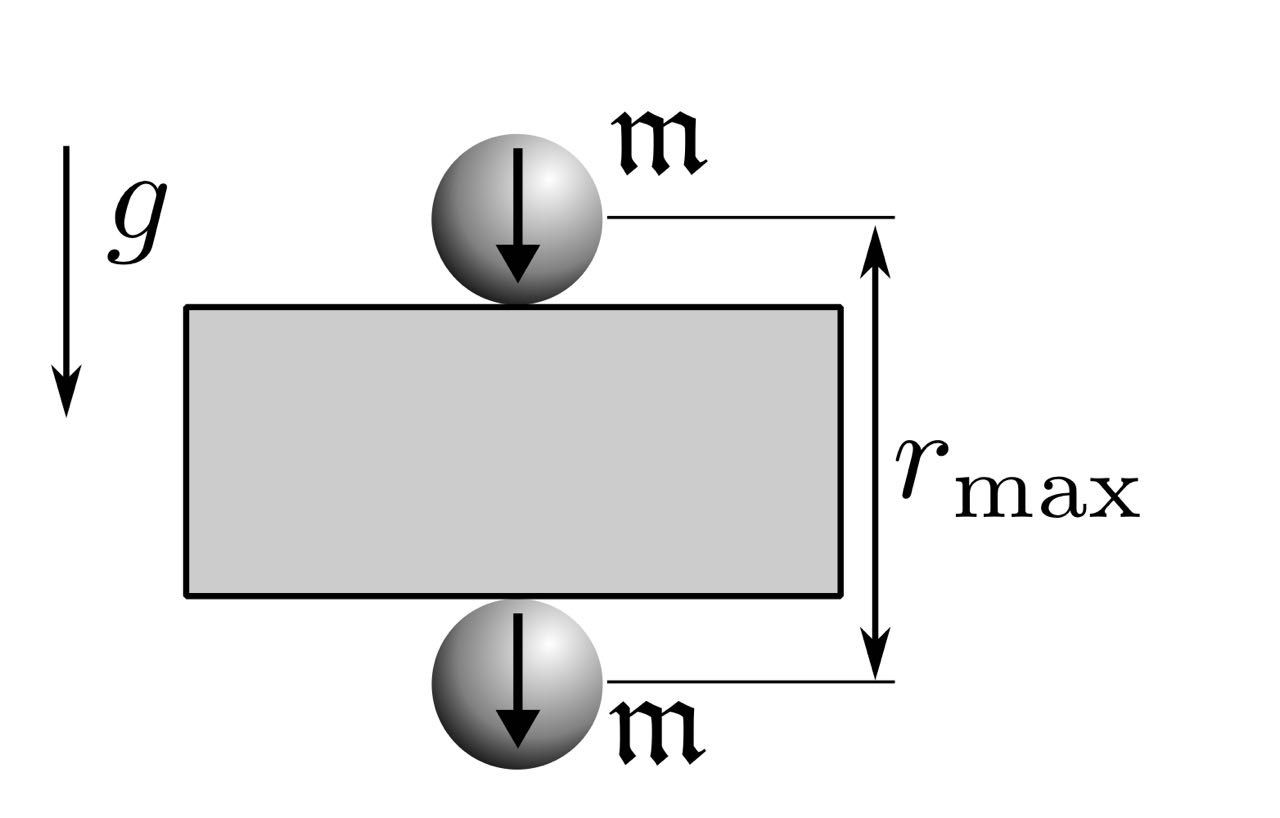
\includegraphics[width=1\textwidth]{3.1.3/rmax.jpg}
    \caption{Измерение магнитных мометов шариков}
\end{center}
\end{wrapfigure}

Когда векторы двух магнитных моментов ориентированы вертикально, из (\ref{6}) имеем

\begin{equation*}
    \mathfrak{m} = \sqrt{\frac{2\pi mgr^4_{max}}{3 \mu_0}} \ \text{(ед. СИ).}
\end{equation*}

По величине $\mathfrak{m}$ с помощью (\ref{2}) можно рассчитать величину индукции $\textbf{B}$ вблизи любой точки на поверхности шара радиуса $R$. Максимальная величина индукции наблюдается на полюсах.

\textbf{Метод Б.} Величину магнитного момента шариков можно определить также по силе их сцепления. Она определяется как сила, необходимая для разрыва двух сцепившихся магнитных шариков. Сила сцепления максимальна, если шары соединяются своими противоположными полюсами (магнитные моменты сонаправлены).

\begin{wrapfigure}{r}{0.3\textwidth}
\begin{center}
    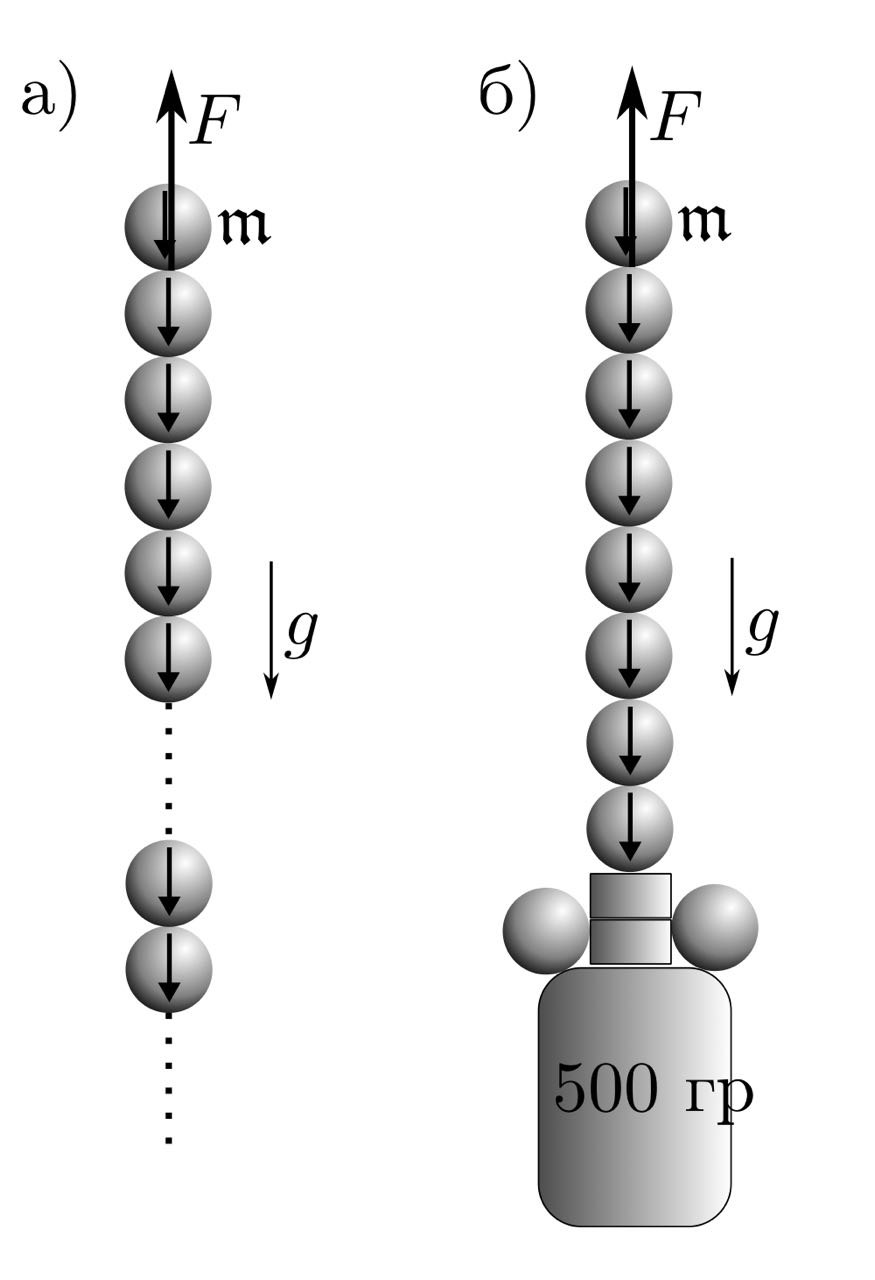
\includegraphics[width=1\textwidth]{3.1.3/mmax.jpg}
    \caption{Альтернативный метод измерения магнитных мометов шариков}
\end{center}
\end{wrapfigure}


Максимальную силу сцепления можно определить по весу магнитной цепочки, которую способен удержать самый верхний магнитный шарик. Если цепь состоит из одинаковых магнитных шариков, то при определённой длине она отрывается от верхнего шарика. При этом, учитывая, что сила притяжения убывает как $F \propto 1/r^4$, где $r$ — расстояния между центрами шаров, для расчёта прочности цепочки достаточно учитывать силу взаимодействия верхнего шара с 3–4 ближайшими соседями.

Сила сцепления двух одинаковых шаров радиусами $R$ с магнитными момантами $\mathfrak{m}$ равна 

\begin{equation*}
        F_0 = \frac{3 \mu_0 \mathfrak{m}^2}{32 \pi R^4}\  \text{(ед. СИ).}    
\end{equation*}

\hfill \break
Тогда минимальный вес цепочки, при котором она оторвётся от верхнего шарика, равен

\begin{equation*}
    F = F_0\left(1 + \frac{1}{2^4} + \frac{1}{3^4} + ... \right) \approx 1,08F_0.
\end{equation*}

\hfill \break
Отметим, что не обязательно составлять цепочку только из одинаковых шариков: на расстояниях, превышающих 20–30 диаметров шариков, можно подцепить любой груз, притягиваемый магнитом, на результат это не повлияет, в чём несложно убедиться экспериментально.

\section{Результаты измерений и обработка данных}

В начале были проведены подготовительные измерения, данные которых приведены в таблице \ref{prep}.

\floatsetup[table]{capposition=top}
\begin{table}[H]
    \centering
    \begin{tabular}{|c|c|c|}
        \hline $d$, см & $m$, г & $B_{p1}$, мТл \\ \hline
          0,6 \pm 0,001   & 0,842 \pm 0,001 &  231 \pm 0,5  \\ \hline
    \end{tabular}
    \caption{Подготовительные измерения}
    \label{prep}
\end{table}

Далее, путём подкладывания листов бумаги было отпределено значение $r_{max} = 1,78 \pm 0,05$ см, максимальное расстояние на котором шарики удерживают друг друга в поле тяжести Земли. Масса отрывающейся цепочки оказалось равной $m_{\text{цеп}}=212,4 \pm 1 г$ г. По этим данным были рассчитаны значения $\mathfrak{m}_1 = 3,7 \pm 0,05 \cdot 10^{-2} \text{Дж}/\text{Тл} 
$ и $\mathfrak{m}_2 = 6,5 \pm 0,04 \cdot 10^{-2} \text{Дж}/\text{Тл}$. По измерениям магнитного поля магнитным момент оказался равным $\mathfrak{m}_1 = 3,1 \pm 0,01 \cdot 10^{-2} \text{Дж}/\text{Тл}$, откуда можно заключить, что более точным оказался первый способ.

Была собрана установка для измерения периода малых колебаний магнитной стрелки (рис. \ref{horiz}). Данные измерений приведены в таблице \ref{tn}.

\begin{figure}[H]
    \centering
    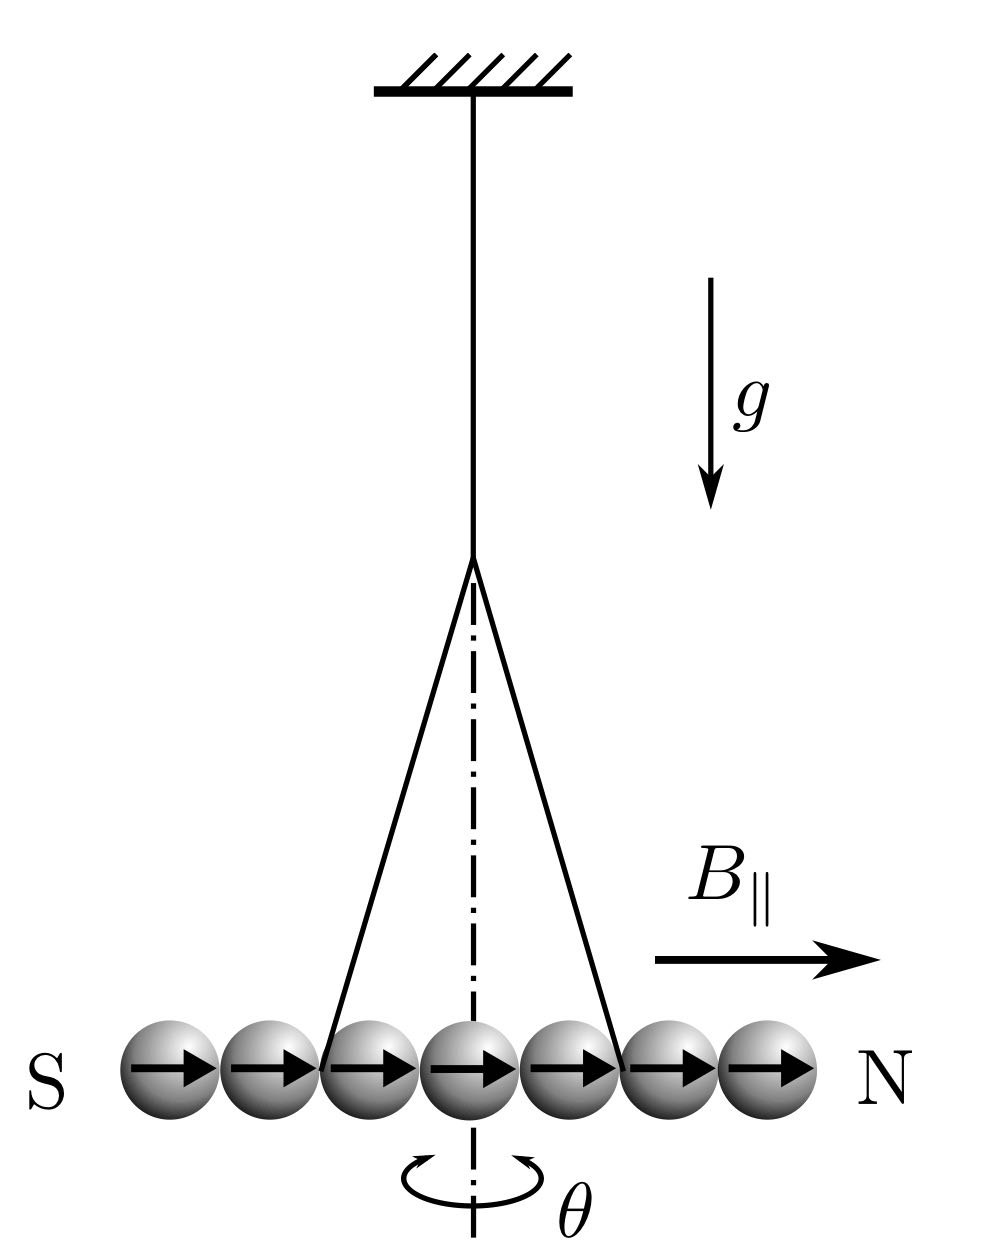
\includegraphics[scale=0.15]{3.1.3/horiz.jpg}
    \label{horiz}
    \caption{Крутильный маятник во внешнем магнитном поле}
\end{figure}

\begin{table}[h]
    \centering
    \begin{tabular}{|c|c|c|c|c|}
    \hline  $n_{\text{шар}}$ & $n_{\text{колеб}}$ & $t$, с & $T$, с & $\varepsilon_T$, \%\\ \hline
        11 & 6 &  23, 6 & 3, 93 & 2 \\ \hline
        9  & 6 &  19, 7 & 3, 28 & 2 \\ \hline
        8  & 8 &  23, 3 & 2, 91 & 2 \\ \hline
        7  & 9 &  22, 7 & 2, 52 & 2 \\ \hline
        6  & 8 &  17, 1 & 2, 13 & 2 \\ \hline
        5  & 8 &  14, 2 & 1, 78 & 2 \\ \hline
        4  & 10 & 14, 4 & 1, 44 & 2 \\ \hline
    \end{tabular}
    \caption{Зависимость периода колебаний от количества шариков в магнитной стрелке}
    \label{tn}
\end{table}

По данным измерений был построен график (\ref{time}).

\begin{figure}[H]
    \centering
    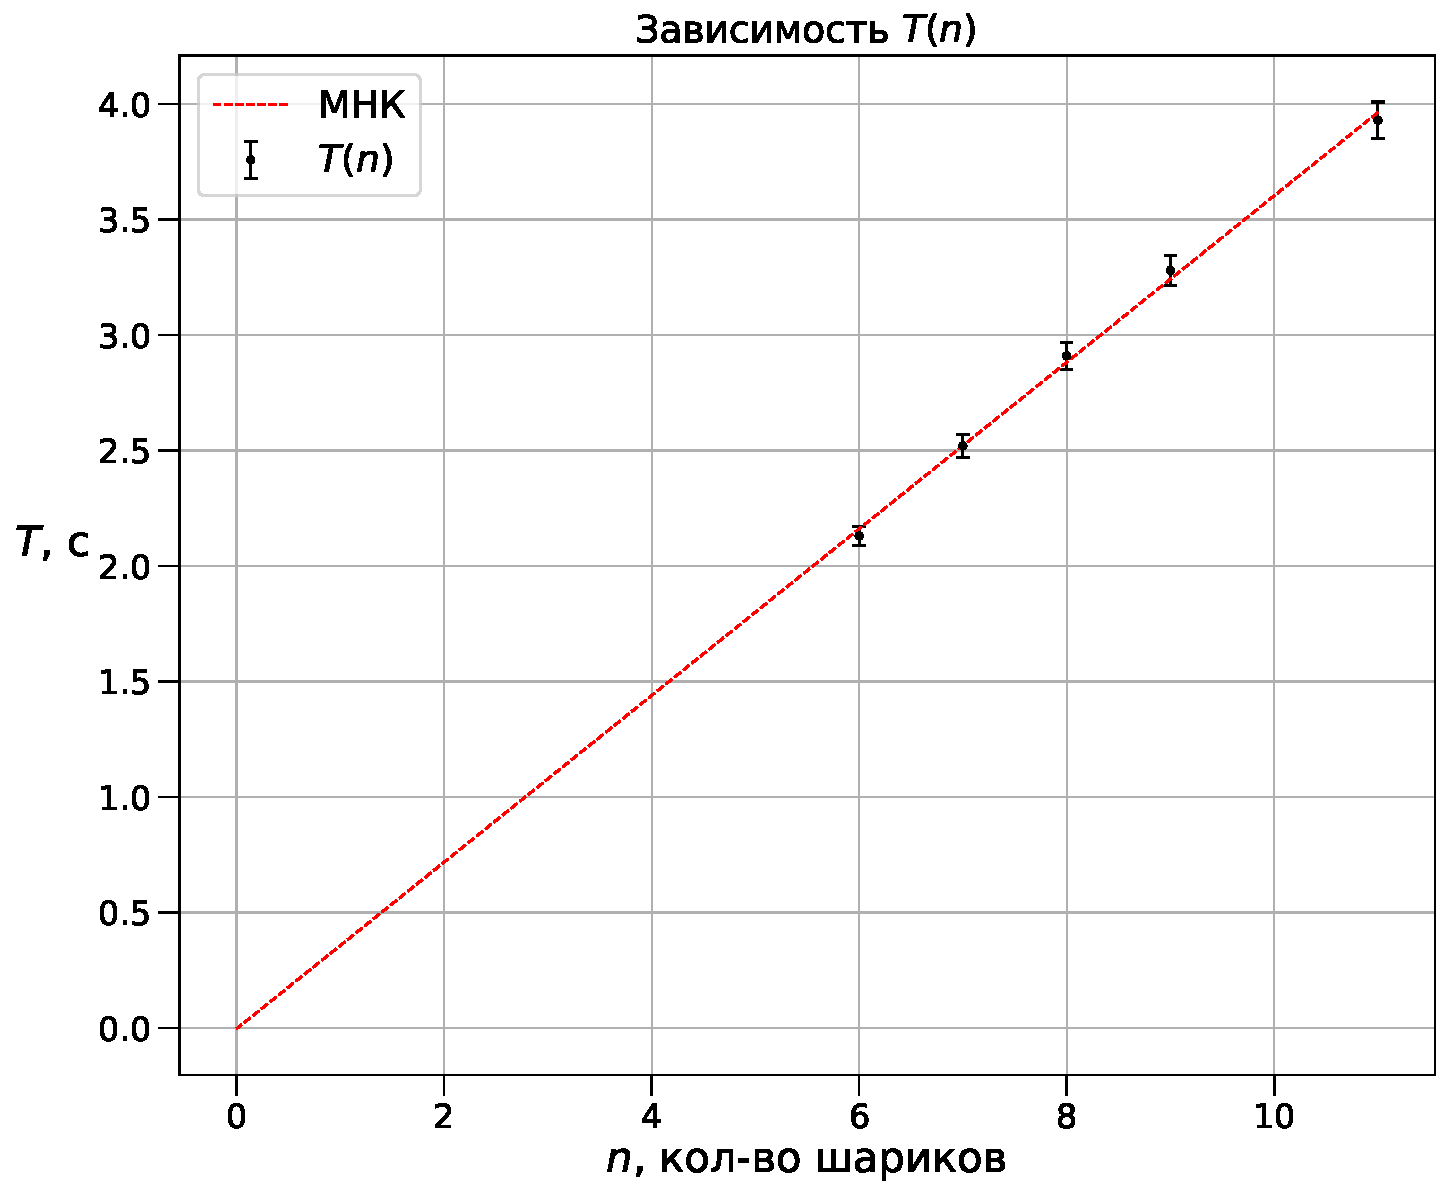
\includegraphics[scale=0.65]{3.1.3/T(n).pdf}
    \caption{\centering{График зависимости периода колбебаний от количества шариков в магнитной стрелке}}
    \label{time}
\end{figure}

По углу наклона несложно определить горизонтальную составляющую магнитного поля Земли, которая оказалась равна  $B_h = 2,48 \pm 0,12 \cdot 10^{-5} \text{Тл}$.

\begin{equation*}
    T(n) = 2\pi \sqrt{\frac{mR^2}{3 \mathfrak{m} B_{h}}} \cdot n.
\end{equation*}

Для следующих измерений был определен диаметр маленького магнитного шарика. Он составил $r_m = 4,63$ см. Далее, для определения вертикальной составляющей магнитного поля Земли была собрана другая установка (рис. \ref{vert}).

\begin{figure}[H]
    \centering
    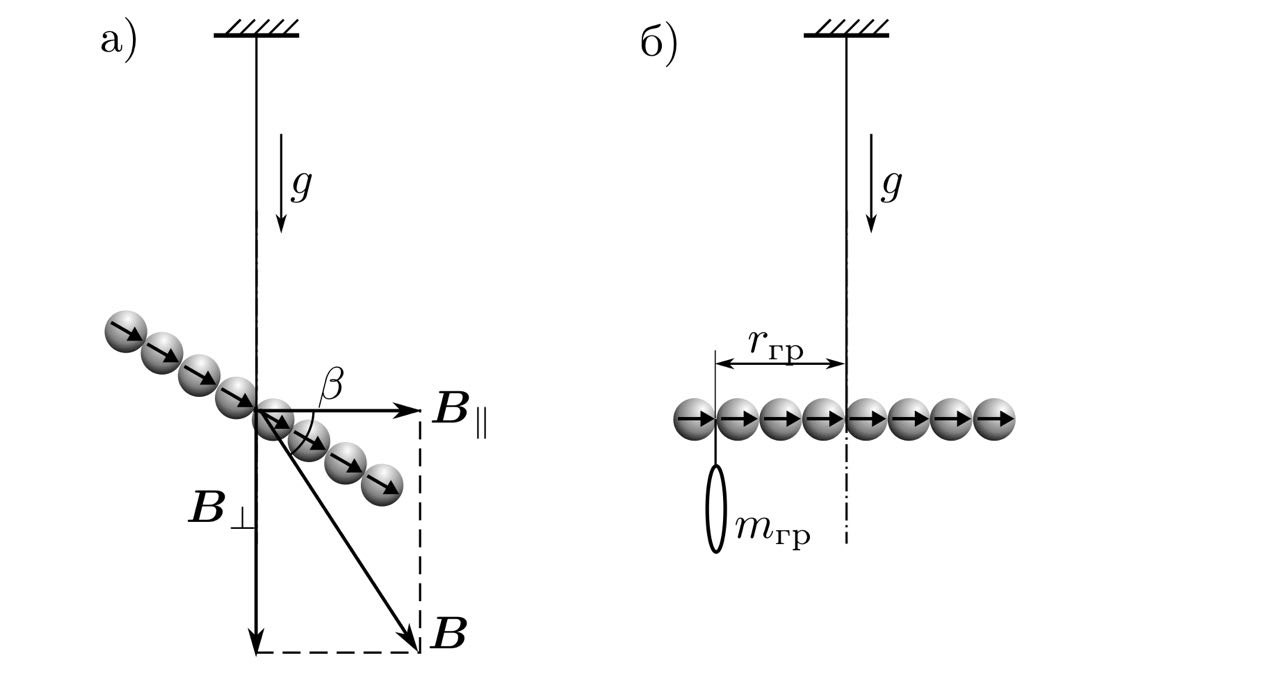
\includegraphics[scale=0.21]{3.1.3/vert.jpg}
    \caption{Измерение вертикальной составляющей поля и магнитного наклонения}
    \label{vert}
\end{figure}

Далее, уравновешиванием кусочками проволки мы приводили стрелку в горизонтальное положение. Данные моментов приведены в таблице \ref{moment}.

\begin{table}[H]
    \centering
    \begin{tabular}{|c|c|c|c|}
        \hline $M$, $r_{\text{ш}}g$ г & $n_{\text{шар}}$ & $M$, мкН$\cdot$м & $\varepsilon_M$ \\ \hline 
        0,92 & 12 & 418 & 5 \\ \hline
        0,69 & 10 & 314 & 5 \\ \hline
        0,46 & 8  & 209 & 5 \\ \hline
        0,42 & 6  & 191 & 5 \\ \hline
        0,33 & 4  & 150 & 5 \\ \hline
    \end{tabular}
    \caption{Зависимость момента от количества шариков в <<магнитной стрелке>>}
    \label{moment}
\end{table}

По полученным данным был построен график (\ref{mn}).

\begin{figure}[H]
    \centering
    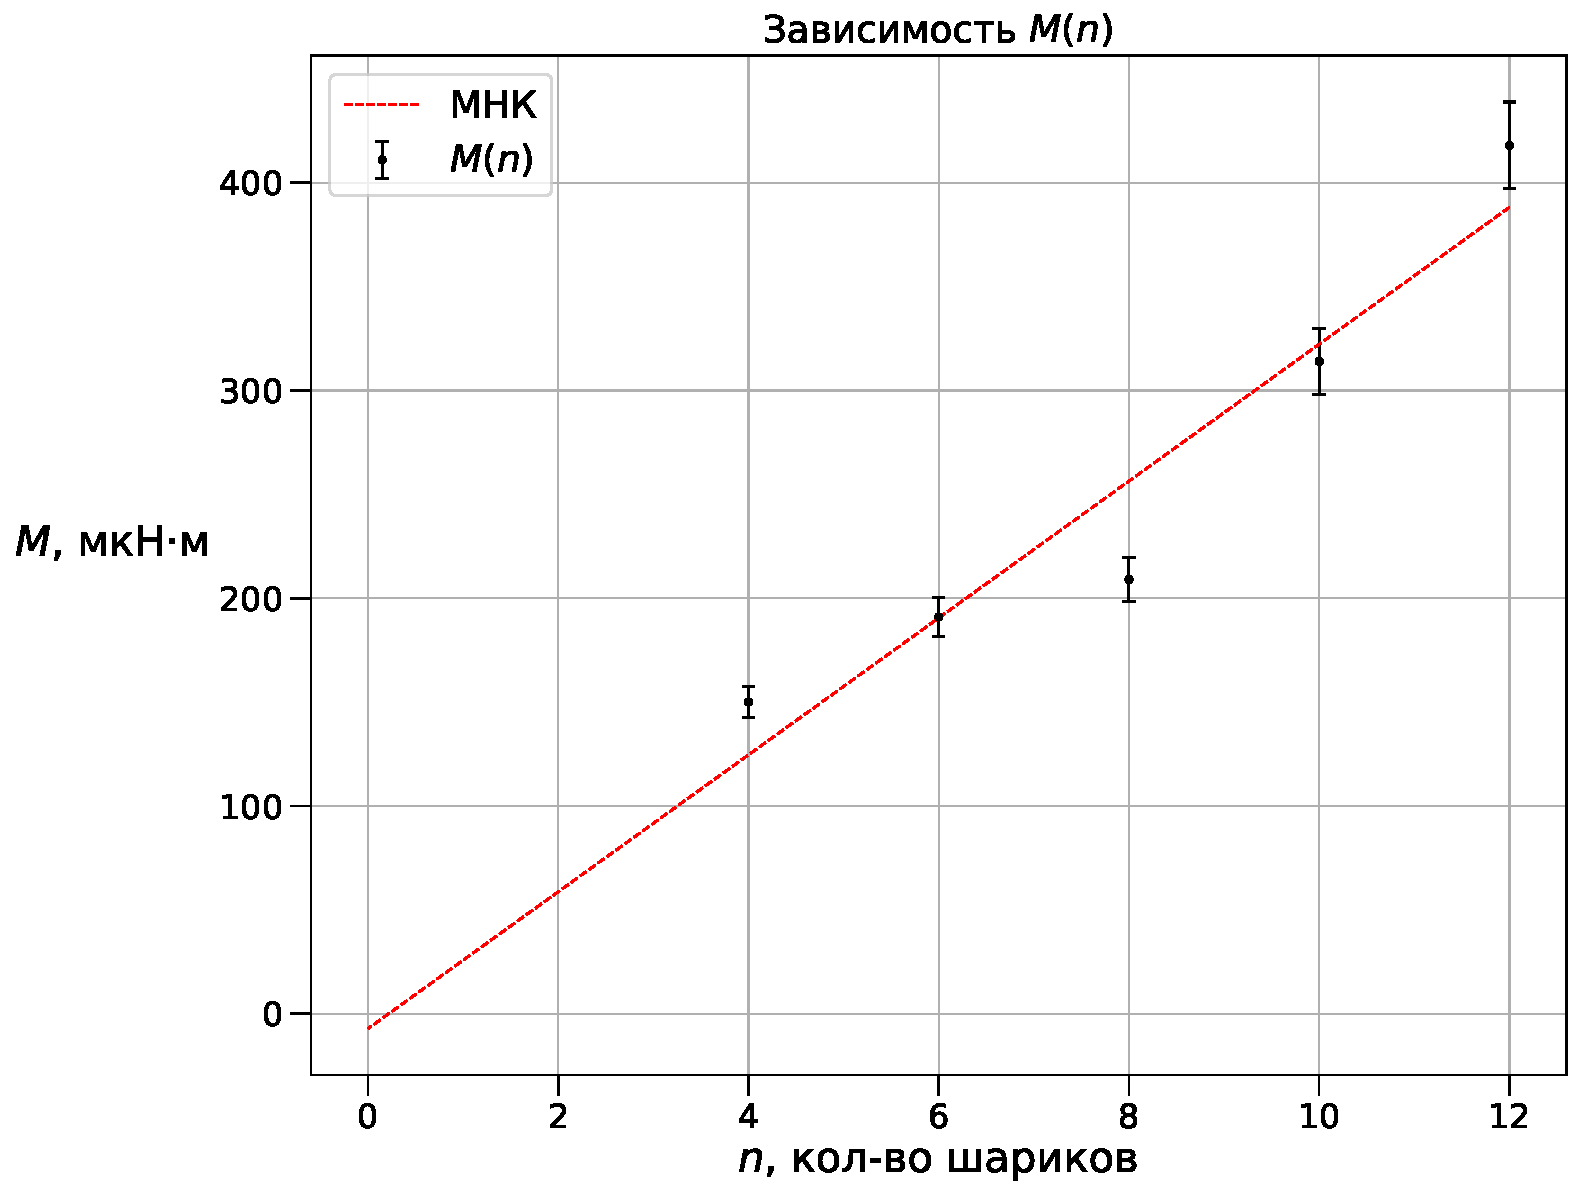
\includegraphics[scale=0.65]{3.1.3/M(n).pdf}
    \caption{График зависимоти момента силы тяжести от количества шариков}
    \label{mn}
\end{figure}

По графику видно, что данные плохо ложатся на прямую даже в пределах погрешности. Это обусловлено тем, что набор возможных грузов и, соответственно, моментов дискретен и не может быть подобран более точно, из-за чего и выбивается из теоретической погрешности.
По наклону фитирующей прямой была вычеслена вертикальная компонента магнитного поля земли, которая составила $B_v = \frac{M}{n\mathfrak{m}} = 3,30 \pm 0,44 \cdot 10^{-5} \text{Тл}$.

Табличные данные магнитного поля в Москве приведены ниже:
\begin{center}
\centering
    $B_{\text{табл}} = 5 \cdot 10^{-5} \text{Тл}$ \break
    $B_{\text{эксп}} = 4,14 \cdot 10^{-5} \text{Тл}$
    
\end{center}



\end{document}
